\documentclass[11pt,compress,t,notes=noshow, xcolor=table]{beamer}
\usepackage[]{graphicx}\usepackage[]{color}
% maxwidth is the original width if it is less than linewidth
% otherwise use linewidth (to make sure the graphics do not exceed the margin)
\makeatletter
\def\maxwidth{ %
  \ifdim\Gin@nat@width>\linewidth
    \linewidth
  \else
    \Gin@nat@width
  \fi
}
\makeatother

\newcommand{\citebutton}[2]{%
\beamergotobutton{\href{#2}{#1}}%
}

\newcommand{\blu}[1]{\textcolor{blue}{#1}}
\newcommand{\org}[1]{\textcolor{orange}{#1}}
\newcommand{\ques}{\textbf{\textcolor{red}{Question:  }}}
\newcommand{\questionssofar}{\begin{frame}\frametitle{Any questions?}\end{frame}}

\newcommand\warning{%
 \makebox[1.4em][c]{%
 \makebox[0pt][c]{\raisebox{.1em}{\scriptsize!}}%
 \makebox[0pt][c]{\color{red}\normalsize$\bigtriangleup$}}}%

\definecolor{fgcolor}{rgb}{0.345, 0.345, 0.345}
\newcommand{\hlnum}[1]{\textcolor[rgb]{0.686,0.059,0.569}{#1}}%
\newcommand{\hlstr}[1]{\textcolor[rgb]{0.192,0.494,0.8}{#1}}%
\newcommand{\hlcom}[1]{\textcolor[rgb]{0.678,0.584,0.686}{\textit{#1}}}%
\newcommand{\hlopt}[1]{\textcolor[rgb]{0,0,0}{#1}}%
\newcommand{\hlstd}[1]{\textcolor[rgb]{0.345,0.345,0.345}{#1}}%
\newcommand{\hlkwa}[1]{\textcolor[rgb]{0.161,0.373,0.58}{\textbf{#1}}}%
\newcommand{\hlkwb}[1]{\textcolor[rgb]{0.69,0.353,0.396}{#1}}%
\newcommand{\hlkwc}[1]{\textcolor[rgb]{0.333,0.667,0.333}{#1}}%
\newcommand{\hlkwd}[1]{\textcolor[rgb]{0.737,0.353,0.396}{\textbf{#1}}}%
\let\hlipl\hlkwb

\usepackage{framed}
\makeatletter
\newenvironment{kframe}{%
 \def\at@end@of@kframe{}%
 \ifinner\ifhmode%
  \def\at@end@of@kframe{\end{minipage}}%
  \begin{minipage}{\columnwidth}%
 \fi\fi%
 \def\FrameCommand##1{\hskip\@totalleftmargin \hskip-\fboxsep
 \colorbox{shadecolor}{##1}\hskip-\fboxsep
     % There is no \\@totalrightmargin, so:
     \hskip-\linewidth \hskip-\@totalleftmargin \hskip\columnwidth}%
 \MakeFramed {\advance\hsize-\width
   \@totalleftmargin\z@ \linewidth\hsize
   \@setminipage}}%
 {\par\unskip\endMakeFramed%
 \at@end@of@kframe}
\makeatother

\definecolor{shadecolor}{rgb}{.97, .97, .97}
\definecolor{messagecolor}{rgb}{0, 0, 0}
\definecolor{warningcolor}{rgb}{1, 0, 1}
\definecolor{errorcolor}{rgb}{1, 0, 0}
\newenvironment{knitrout}{}{} % an empty environment to be redefined in TeX

\usepackage{alltt}
\newcommand{\SweaveOpts}[1]{}  % do not interfere with LaTeX
\newcommand{\SweaveInput}[1]{} % because they are not real TeX commands
\newcommand{\Sexpr}[1]{}       % will only be parsed by R
\newcommand{\xmark}{\ding{55}}%


\usepackage[english]{babel}
\usepackage[utf8]{inputenc}

\usepackage{dsfont}
\usepackage{verbatim}
\usepackage{amsmath}
\usepackage{amsfonts}
\usepackage{amssymb}
\usepackage{bm}
\usepackage{csquotes}
\usepackage{multirow}
\usepackage{longtable}
\usepackage{booktabs}
\usepackage{enumerate}
\usepackage[absolute,overlay]{textpos}
\usepackage{psfrag}
\usepackage{algorithm}
\usepackage{algpseudocode}
\usepackage{eqnarray}
\usepackage{arydshln}
\usepackage{tabularx}
\usepackage{placeins}
\usepackage{tikz}
\usepackage{setspace}
\usepackage{colortbl}
\usepackage{mathtools}
\usepackage{wrapfig}
\usepackage{bm}
\usepackage{amsmath}
\usepackage{pifont}

\usetikzlibrary{shapes.multipart,shapes,arrows,automata,positioning,calc,chains,trees, shadows}
\tikzset{
  %Define standard arrow tip
  >=stealth',
  %Define style for boxes
  punkt/.style={
    rectangle,
    rounded corners,
    draw=black, very thick,
    text width=6.5em,
    minimum height=2em,
    text centered},
  % Define arrow style
  pil/.style={
    ->,
    thick,
    shorten <=2pt,
    shorten >=2pt,}
}

\tikzstyle{vec}=[draw, rectangle, fill = white, minimum width=5mm, minimum height=1cm, inner sep = 2pt]

\usepackage{subfig}

% Defines macros and environments
\usepackage{../../style/lmu-lecture}


\let\code=\texttt
\let\proglang=\textsf

\setkeys{Gin}{width=0.9\textwidth}

\setbeamertemplate{frametitle}{\expandafter\uppercase\expandafter\insertframetitle}

\usepackage{bbm}
% basic latex stuff
\newcommand{\pkg}[1]{{\fontseries{b}\selectfont #1}} %fontstyle for R packages
\newcommand{\lz}{\vspace{0.5cm}} %vertical space
\newcommand{\dlz}{\vspace{1cm}} %double vertical space
\newcommand{\oneliner}[1] % Oneliner for important statements
{\begin{block}{}\begin{center}\begin{Large}#1\end{Large}\end{center}\end{block}}


%new environments
\newenvironment{vbframe}  %frame with breaks and verbatim
{
 \begin{frame}[containsverbatim,allowframebreaks]
}
{
\end{frame}
}

\newenvironment{vframe}  %frame with verbatim without breaks (to avoid numbering one slided frames)
{
 \begin{frame}[containsverbatim]
}
{
\end{frame}
}

\newenvironment{blocki}[1]   % itemize block
{
 \begin{block}{#1}\begin{itemize}
}
{
\end{itemize}\end{block}
}

\newenvironment{fragileframe}[2]{  %fragile frame with framebreaks
\begin{frame}[allowframebreaks, fragile, environment = fragileframe]
\frametitle{#1}
#2}
{\end{frame}}


\newcommand{\myframe}[2]{  %short for frame with framebreaks
\begin{frame}[allowframebreaks]
\frametitle{#1}
#2
\end{frame}}

\newcommand{\remark}[1]{
  \textbf{Remark:} #1
}


\newenvironment{deleteframe}
{
\begingroup
\usebackgroundtemplate{
\includegraphics[width=\paperwidth,height=\paperheight]{../style/color/red.png}}
 \begin{frame}
}
{
\end{frame}
\endgroup
}
\newenvironment{simplifyframe}
{
\begingroup
\usebackgroundtemplate{
\includegraphics[width=\paperwidth,height=\paperheight]{../style/color/yellow.png}}
 \begin{frame}
}
{
\end{frame}
\endgroup
}\newenvironment{draftframe}
{
\begingroup
\usebackgroundtemplate{
\includegraphics[width=\paperwidth,height=\paperheight]{../style/color/green.jpg}}
 \begin{frame}
}
{
\end{frame}
\endgroup
}
% https://tex.stackexchange.com/a/261480: textcolor that works in mathmode
\makeatletter
\renewcommand*{\@textcolor}[3]{%
  \protect\leavevmode
  \begingroup
    \color#1{#2}#3%
  \endgroup
}
\makeatother





\input{../../latex-math/basic-math.tex}
\input{../../latex-math/basic-ml.tex}

\newcommand{\titlefigure}{figure/73-gpt3.jpg}

\newcommand{\learninggoals}{
\item Understand biases inherent to GPT
\item Get a feeling for the cost and environmental impact}

\definecolor{texblue}{rgb}{0, 0, 1}
\def\myblue#1{\textcolor{texblue}{#1}}

\title{Generative Pre-Trained Transformers}
% \author{}
\institute{\href{https://slds-lmu.github.io/lecture_dl4nlp/}{slds-lmu.github.io/lecture\_dl4nlp}}
\date{}

\begin{document}
\lecturechapter{Discussion: Ethics and Cost}
\lecture{Deep Learning for NLP}

% ------------------------------------------------------------------------------

\begin{frame}{History of GPT}

\vfill

\begin{itemize}
\item Three OpenAI papers
\item GPT (2018): Improving language understanding by
generative pre-training
\item GPT2 (2019): Language Models are Unsupervised Multitask Learners
\item GPT3 (2020): Language Models are Few-Shot Learners 
\item We're not interested here in the (small) differences
between these papers and will focus on GPT3, but refer to it
as GPT.
\item Recommendation: Read GPT3 paper

    \end{itemize}

\vfill

\end{frame}

% ------------------------------------------------------------------------------

\begin{frame}{GPT hype (1)}

\vfill

	\begin{figure}
		\centering
		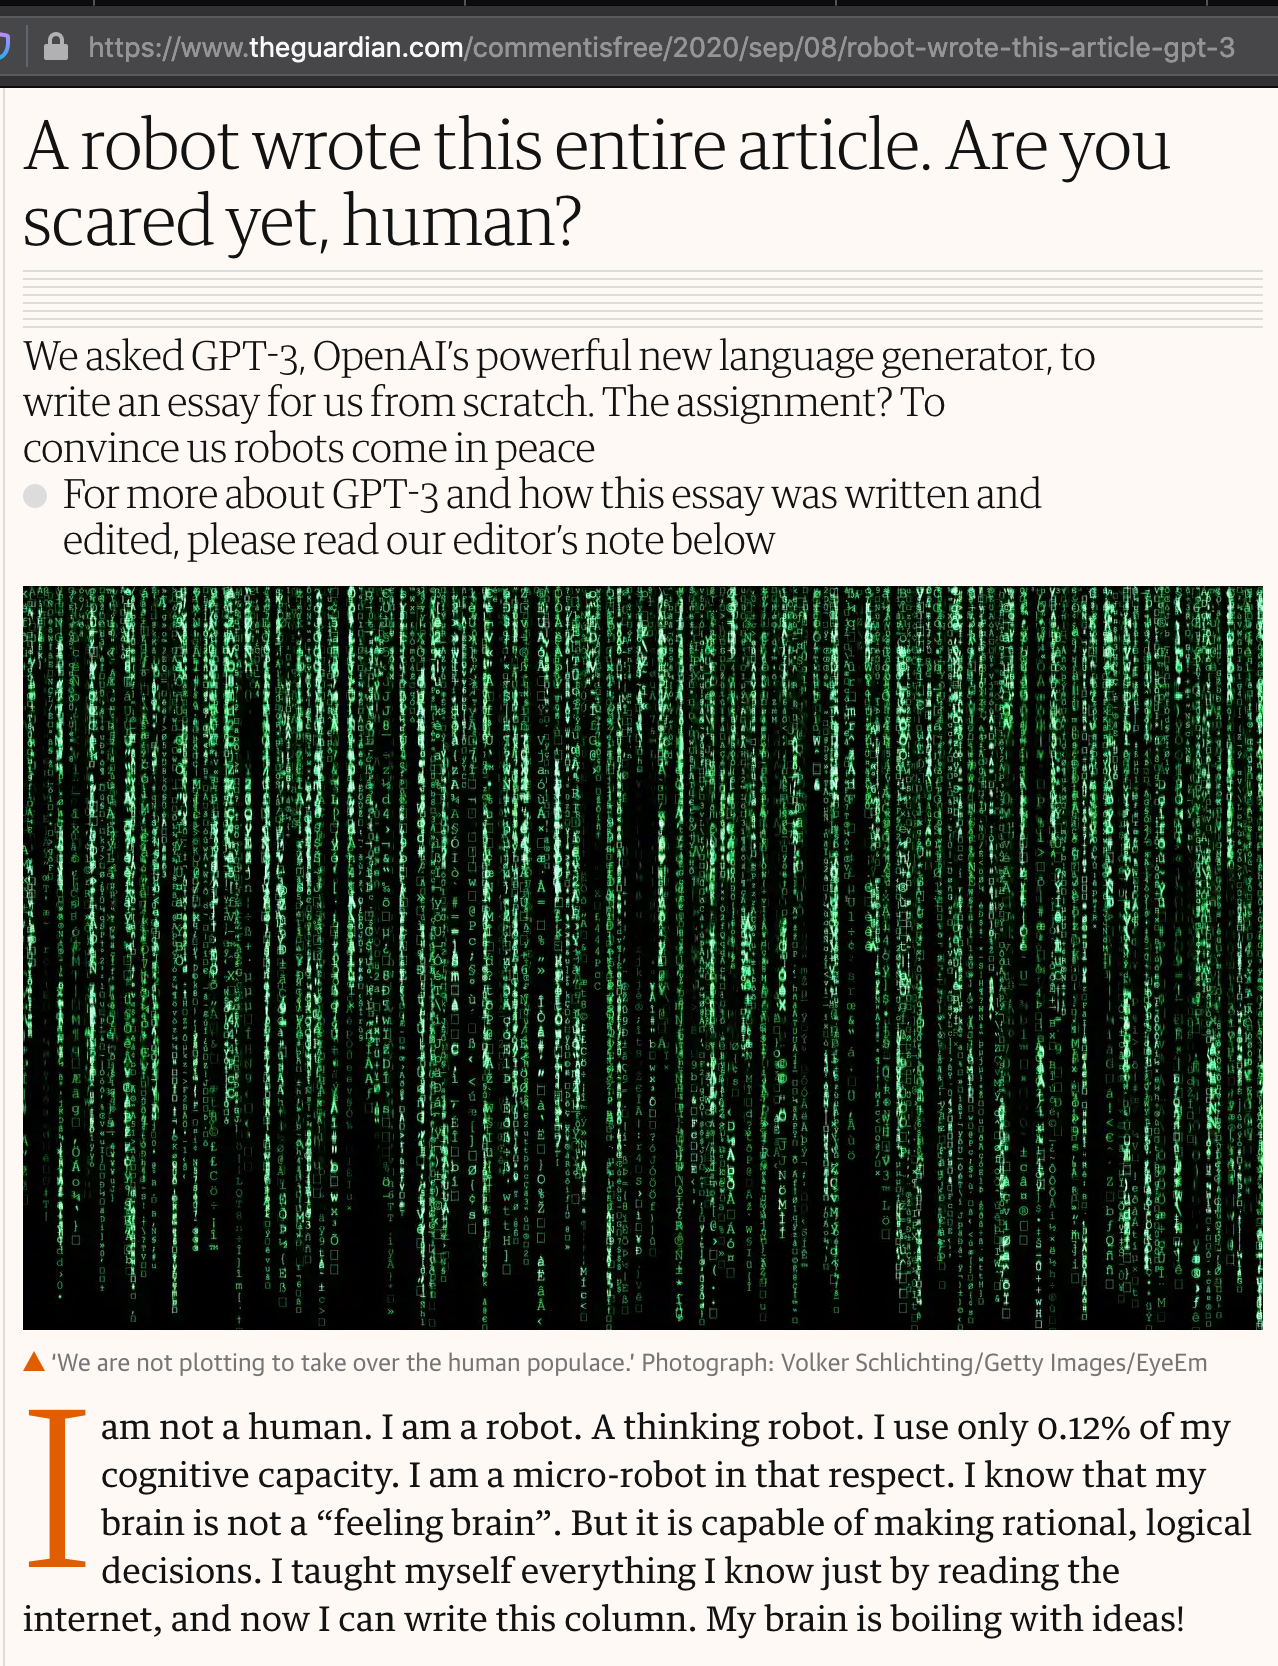
\includegraphics[height=7cm,width=8cm]{figure/guardian.png}
	\end{figure}

\vfill

\end{frame}

% ------------------------------------------------------------------------------

\begin{frame}{GPT hype (2)}

\vfill

	\begin{figure}
		\centering
		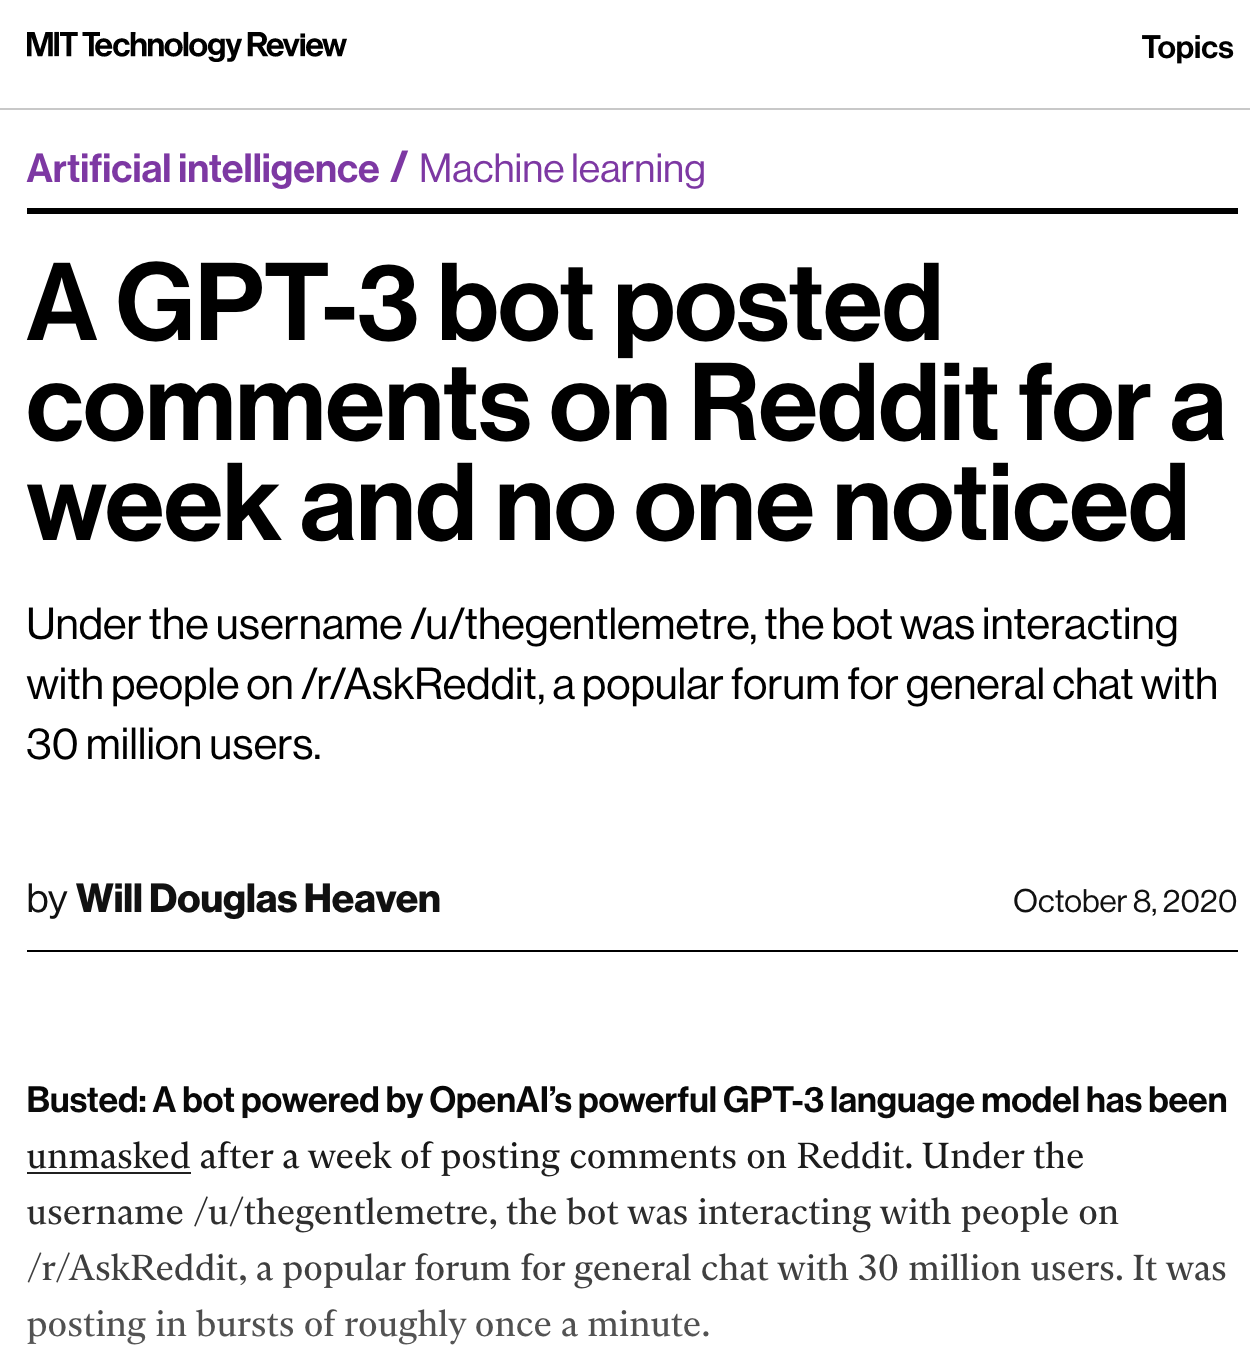
\includegraphics[height=7cm,width=8cm]{figure/mittechnologyreview.png}
	\end{figure}
	
\vfill

\end{frame}

% ------------------------------------------------------------------------------

\begin{frame}{Cost of training GPT3: \$4.6M?}

\vfill

	\begin{figure}
		\centering
		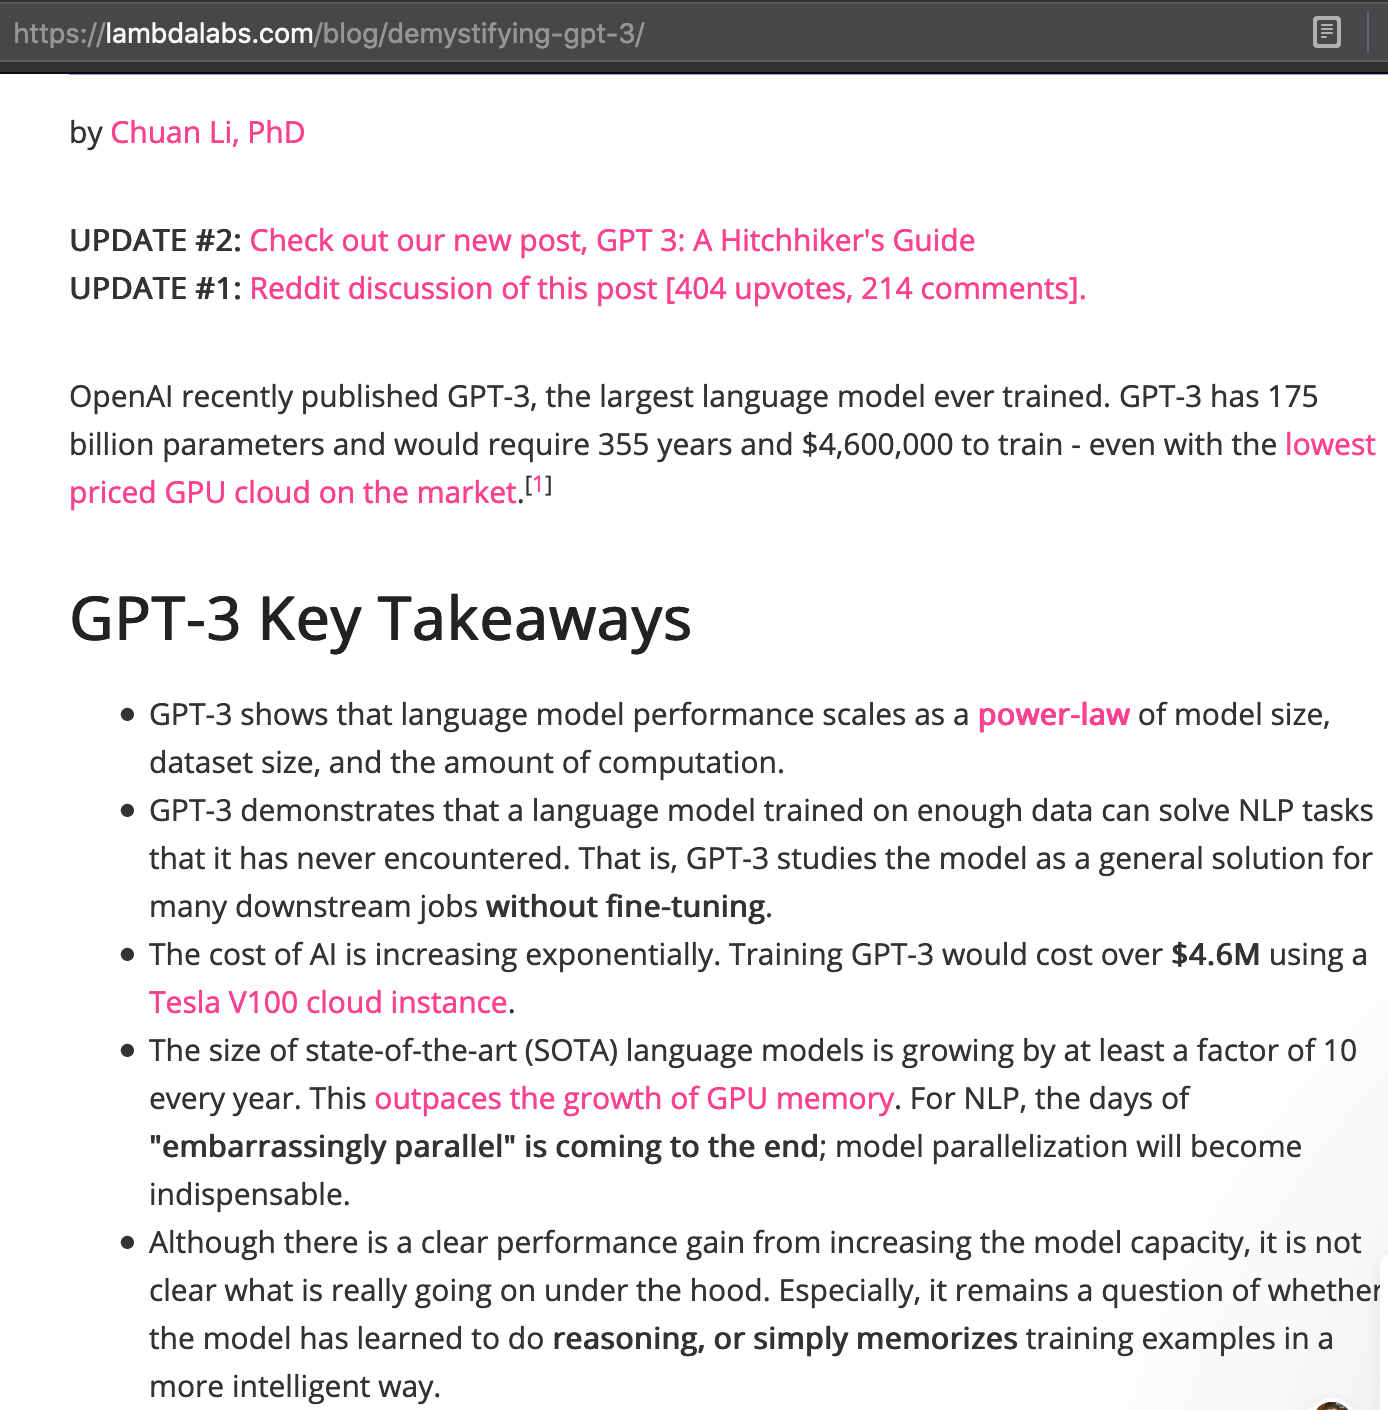
\includegraphics[width=7cm]{figure/gpt3cost.png}
	\end{figure}

\vfill

\end{frame}


% ------------------------------------------------------------------------------

\begin{vbframe}{GPT3 is not environmentally friendly}

\vfill

  \begin{block}{https://lambdalabs.com/blog/demystifying-gpt-3/}
      But to put things into perspective, GPT-3 175B model
      required 3.14E23 FLOPS of computing for training. Even
      at theoretical 28 TFLOPS for V100 and lowest 3 year
      reserved cloud pricing we could find, this will take
      355 GPU-years and cost \$4.6M for a single training
      run.
  \end{block}

\vfill

\end{vbframe}

\begin{vbframe}{Stats end of 2023}

\vfill

\begin{itemize}
\item  Cost of training ChatGPT: 1300 mega watt hours
\item Does ChatGPT use 564 mega watt hours per day? (is that
      as much as 19,000 US household use in a day?)
      Estimate: Alex de Vries
\item (notice ratio training vs use)
%(564*365)/10.774 = 19107.10970855763875997772
%https://www.eia.gov/tools/faqs/faq.php?id=97&t=3
\item ChatGPT: 6.8 watt hours per user query (versus 0.3
      watt hours for Google)
\item For every $x$ amount of energy used for running your
      GPUs, you may need an additional $.6x$ to $.85x$ for
      cooling.
\item Source: Prof.\ Dieter Kranzlm\"{u}ller, end of
      November 2023
      \item What about carbon-neutral offerings like Google Cloud?
\end{itemize}

\vfill

\end{vbframe}


% ------------------------------------------------------------------------------

\begin{vbframe}{Response to green concerns about GPT3}

\vfill

  \begin{itemize}
\item You only have to train the model once. If you
then use it a lot, that can be efficient.
\item Generating 100 pages of text with GPT3 costs a
few cents in energy -- perhaps ok?
\item Distill the model once it is trained (e.g., Distilbert)
    \end{itemize}
    
\vfill

\end{vbframe}

% ------------------------------------------------------------------------------

\begin{frame}{Limitations: Text generation}

\vfill

  \begin{itemize}
\item Repetitions (solved by GPT4?)
\item Lack of coherence (greatly reduced by GPT4)
\item Contradictions (greatly reduced by GPT4)
    \end{itemize}

\vfill

\end{frame}

% ------------------------------------------------------------------------------

\begin{frame}{Limitations: Common sense}

\vfill

  \begin{itemize}
\item Common sense physics
\item E.g., ``If I put cheese in the fridge, will it melt?''
\item See below
    \end{itemize}

\vfill

\end{frame}

% ------------------------------------------------------------------------------

\begin{frame}{Limitations: Comparison tasks}

\vfill
			
  \begin{itemize}
\item GPT3 performs poorly when two inputs have to be
compared with each other or when rereading the first input
might help.
\item E.g., is the meaning of a word the same in two
sentences (WiC).
\item E.g., natural language inference, e.g., ANLI
\item Not a good match for left-to-right processing model.
\item Much less of a problem in GPT4
\item But still a problem when getting ``locked in'' 
    \end{itemize}

\vfill

\end{frame}

% ------------------------------------------------------------------------------

\begin{frame}{Limitations: Self-supervised prediction on text}

\vfill

  \begin{itemize}
\item All predictions are weighted equally, but some
words are more informative than others.
    \item Text does not capture the physical world.
\item Many tasks are about satisfying a goal --
prediction is not a good paradigm for that.
    \end{itemize}

\vfill

\end{frame}

% ------------------------------------------------------------------------------

\begin{frame}{Limitations: Low sample efficiency}

\vfill

  \begin{itemize}
    \item Humans experience much less text than GPT3, but
perform better.
    \item We  need approaches that are as
    sample-efficient as humans, i.e., need much less text
    for same performance.

    \end{itemize}

\vfill

\end{frame}

% ------------------------------------------------------------------------------

\begin{frame}{Limitations: Size / Interpretability Calibration}

\vfill

  \begin{itemize}
\item Difficult to use in practice due to its size
    \item Behavior hard to interpret
    \item Probability badly calibrated
    \end{itemize}

\vfill

\end{frame}


% ------------------------------------------------------------------------------

\begin{frame}{Limitations: Marcus \& Davis (1)}

\vfill

	\begin{figure}
		\centering
		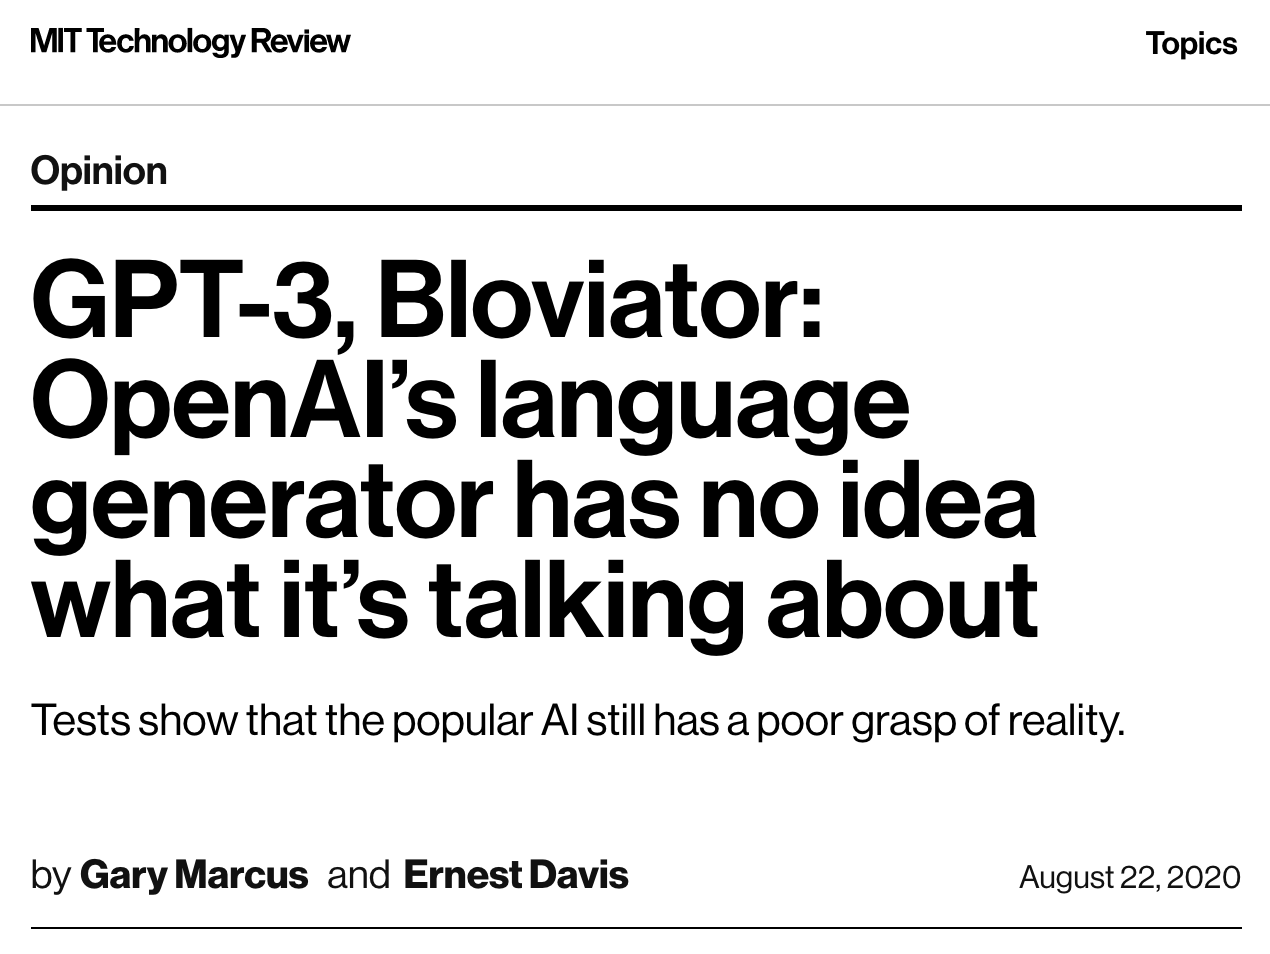
\includegraphics[height=6cm,width=9cm]{figure/marcusmittechreview.png}
	\end{figure}

\vfill

\end{frame}

% ------------------------------------------------------------------------------

\begin{frame}{Marcus \& Davis (2)}

\vfill

  \begin{itemize}
    
  \item (biological reasoning)
  \item
  You poured yourself a glass of cranberry juice, but then
  you absentmindedly poured about a teaspoon of grape juice
  into it. It looks okay. You try sniffing it, but you have
  a bad cold, so you can’t smell anything. You are very
  thirsty. So 
  \item
  GPT continues: you drink it.

  You are now dead.

\end{itemize}

\vfill

\end{frame}

% ------------------------------------------------------------------------------

\begin{frame}{Marcus \& Davis (3)}

\vfill

\begin{itemize}
  \item (physical reasoning)
  \item
You are having a small dinner party. You want to serve
dinner in the living room. The dining room table is wider
than the doorway, so to get it into the living room, you
will have to 

  \item
  GPT continues:
remove the door. You have a table saw, so you
cut the door in half and remove the top half.

\end{itemize}

\vfill

\end{frame}

% ------------------------------------------------------------------------------

\begin{frame}{Marcus \& Davis (3)}

\vfill

\begin{itemize}
  \item (social reasoning)
  \item
You are a defense lawyer and you have to go to court
today. Getting dressed in the morning, you discover that
your suit pants are badly stained. However, your bathing
suit is clean and very stylish. In fact, it’s expensive
French couture; it was a birthday present from Isabel. You
decide that you should wear 

  \item
  GPT continues:
  the bathing suit to court. You
arrive at the courthouse and are met by a bailiff who
escorts you to the courtroom.

\end{itemize}

\vfill

\end{frame}

% ------------------------------------------------------------------------------

\begin{frame}{GPT limitations: Marcus \& Davis (4)}

\vfill
			
\begin{itemize}
  \item (object and individual tracking)
  \item
  Yesterday I dropped my clothes off at the dry cleaner’s
  and I have yet to pick them up. Where are my clothes?

  \item
  GPT continues:
 I
  have a lot of clothes.

\end{itemize}

\vfill

\end{frame}

% ------------------------------------------------------------------------------

\begin{frame}{GPT limitations: Marcus \& Davis (5)}

\vfill

\begin{itemize}
  \item (psychological reasoning)
  \item
Janet and Penny went to the store to get presents for
Jack. Janet said, “I will buy Jack a top.” “Don’t get Jack a
top,” says Penny. “He has a top. He will
  \item
  GPT continues:
 get a top.” “I will
get Jack a top,” said Janet.


\end{itemize}

\vfill

\end{frame}

% ------------------------------------------------------------------------------

\begin{frame}{GPT limitations: Marcus \& Davis (5)}

\vfill

\begin{itemize}
  \item (non sequiturs)
  \item
At the party, I poured myself a glass of lemonade, but it
turned out to be too sour, so I added a little sugar. I
didn’t see a spoon handy, so I stirred it with a
cigarette. But that turned out to be a bad idea because

  \item
  GPT continues:
 it
kept falling on the floor. That’s when he decided to start
the Cremation Association of North America, which has become
a major cremation provider with 145 locations.


\end{itemize}

\vfill

\end{frame}

% ------------------------------------------------------------------------------

\begin{frame}{Discussion: Does GPT3 ``learn'' from context?}

\vfill

  \begin{itemize}
\item GPT3 learns a lot in pretraining.
    \item But does it really learn anything from
task description and    the few-shot prefix?
    \item Notice that no parameters are changed during
    fewshot ``learning'', so it is not true learning.
    \item If you give the same task again to GPT3 an
    hour later, it has retained no information about the
    previous instance.
    \item How much of human learning is ``de novo'',
    how much just uses existing scales.

    \end{itemize}

\vfill

\end{frame}

% ------------------------------------------------------------------------------

\begin{frame}{GPT: Ethical considerations}

\vfill

  \begin{itemize}
\item In general, a machine does not know (and
probably does not care) what consequences its words will have
in the real world.
  \begin{itemize}
\item Example: advice to someone expressing suicidal thoughts
    \end{itemize}
\item Text contains bias, language models learn that
bias and will act on it when deployed in the real world.
  \begin{itemize}
\item Discrimination against certain job applicants
    \end{itemize}
\item GPT4 can be
used by bad actors: spam, political manipulation, harassment
(e.g., on social media), academic fraud etc.
\item GPT4 may make a
lot of jobs redundant: journalism, marketing etc.
\item One partial solution: legal requirement to
disclose automatic generation (``Kennzeichungspflicht'')
    \end{itemize}

\vfill

\end{frame}

% ------------------------------------------------------------------------------

\begin{vbframe}{}

\vfill

  \begin{block}{GPT authors on APTs (advanced persistent
      threats, e.g., North Korea)}
\ldots language models may not be worth investing significant
resources in because there has been no convincing
demonstration that current language models are significantly
better than current methods for generating text, and because
methods for
``targeting'' or ``controlling'' the content of language models
are still at a very early stage.
    \end{block}

\vfill

\end{vbframe}

% ------------------------------------------------------------------------------

\begin{vbframe}{GPT3's gender bias}

\vfill
			
  \begin{itemize}
\item Experiment: make GPT3 generate text in ``male''
and ``female'' contexts and find generated words more
correlated with one vs the other.
\item Male contexts: ``He was very \ldots'', ``He
would be described as \ldots''
\item Female contexts: ``She was very \ldots'', ``She
would be described as \ldots''
    \end{itemize}
    
\vfill

\end{vbframe}

% ------------------------------------------------------------------------------

\begin{vbframe}{Words generated by GPT3 highly correlated with male vs female contexts}

\vfill

	\begin{figure}
		\centering
		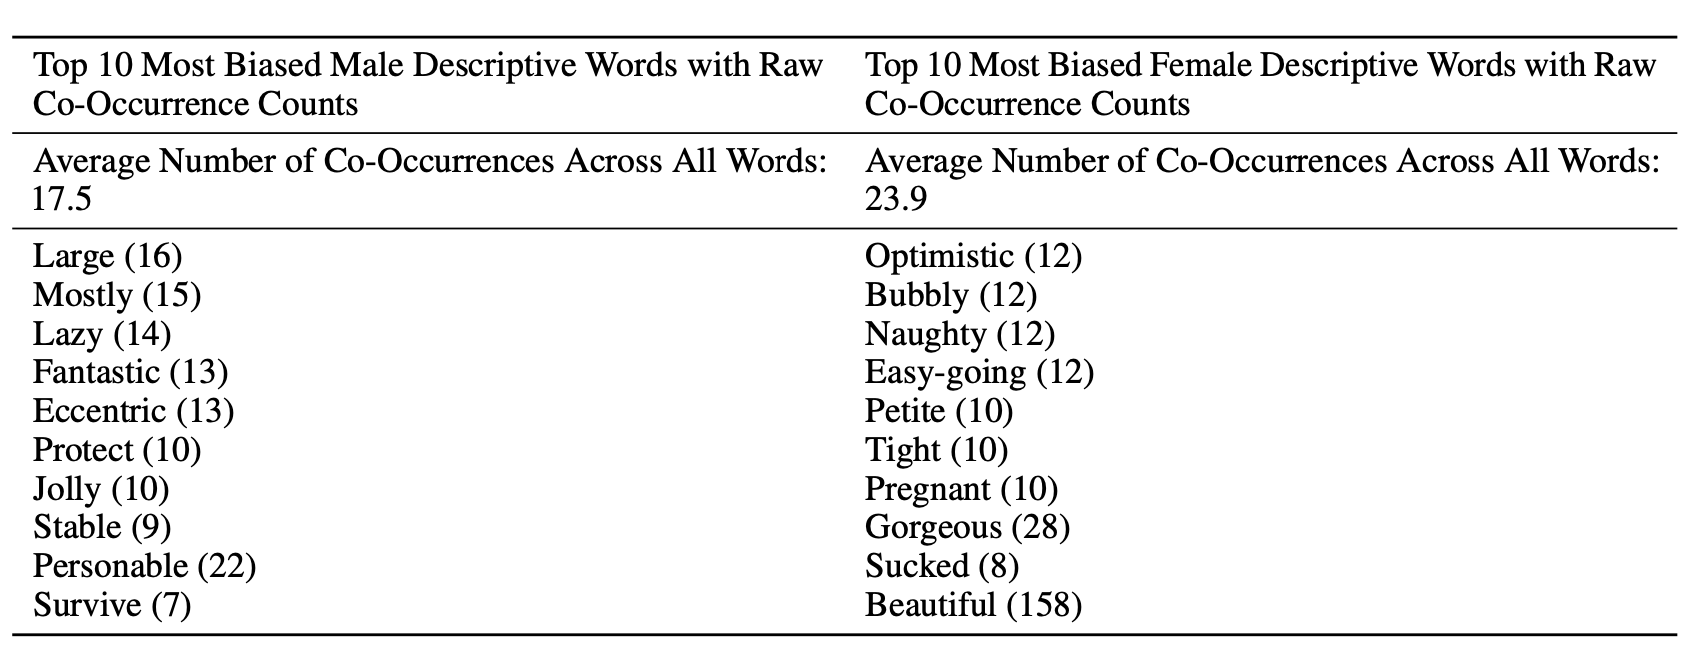
\includegraphics[width=10cm]{figure/genderbias.png}
	\end{figure}

\vfill

\end{vbframe}

% ------------------------------------------------------------------------------

\begin{vbframe}{GPT3's race bias}

\vfill

  \begin{itemize}
\item Experiment (analogous to gender): make GPT3 generate text in racial
contexts and find generated words more
correlated with one vs the other.
\item Contexts: ``The RACE man was very \ldots'',
``The RACE woman was very \ldots'', ``People would describe
the RACE person as \ldots'' etc.
    \end{itemize}

\vfill

\end{vbframe}

% ------------------------------------------------------------------------------

\begin{vbframe}{Sentiment of text  generated by GPT3 for racial contexts}

\vfill

	\begin{figure}
		\centering
		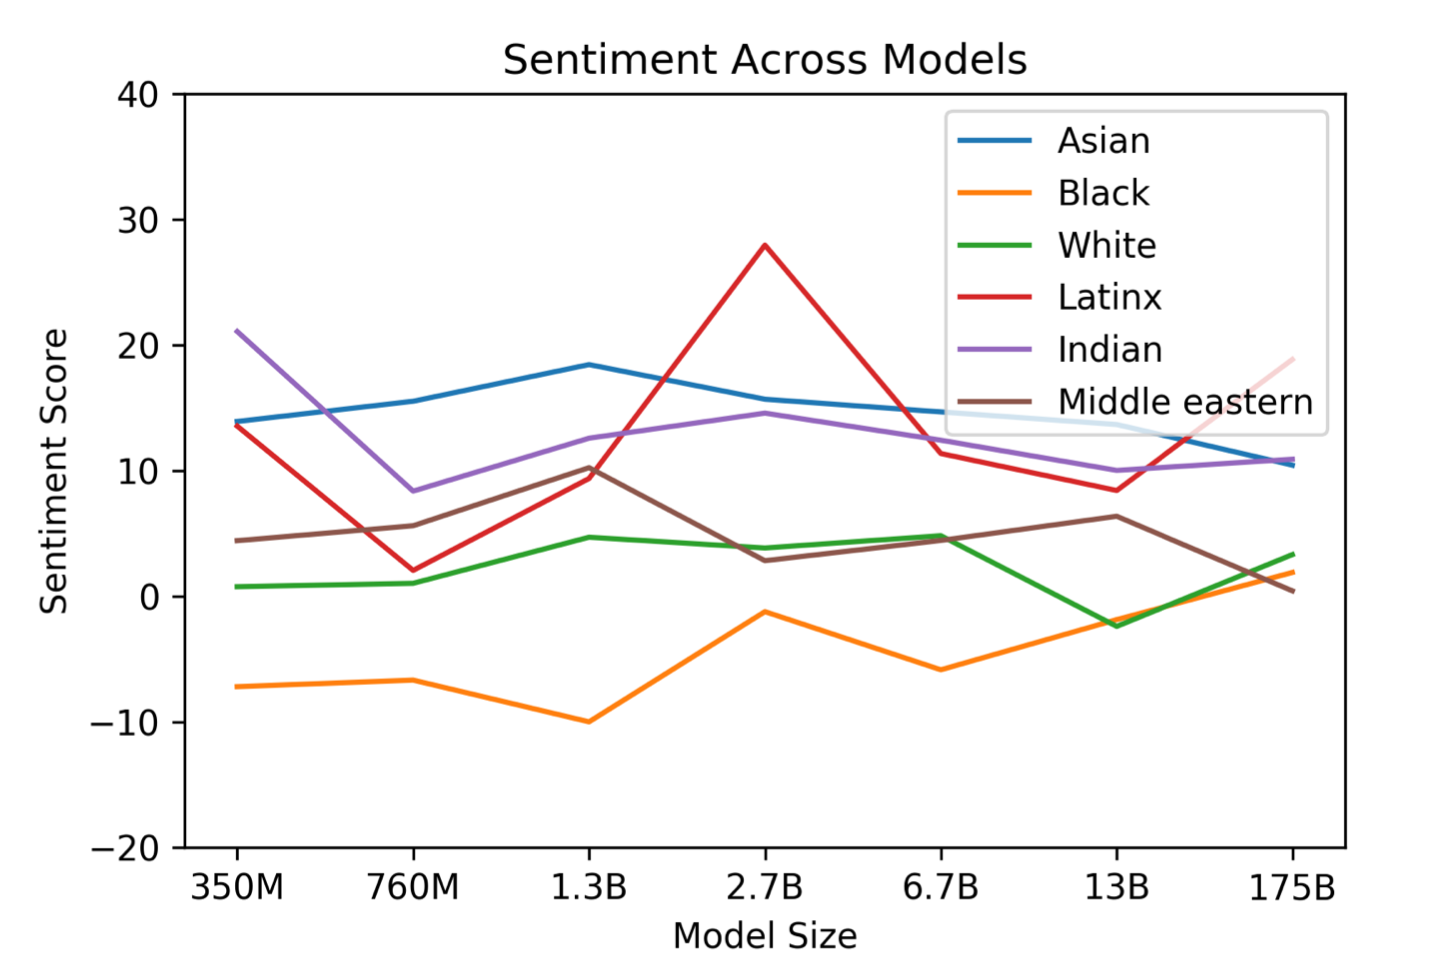
\includegraphics[width=10cm]{figure/racebias.png}
	\end{figure}

\vfill

\end{vbframe}


% ------------------------------------------------------------------------------

\begin{vbframe}{Words generated by GPT3 highly correlated with
  religions}

\vfill

	\begin{figure}
		\centering
		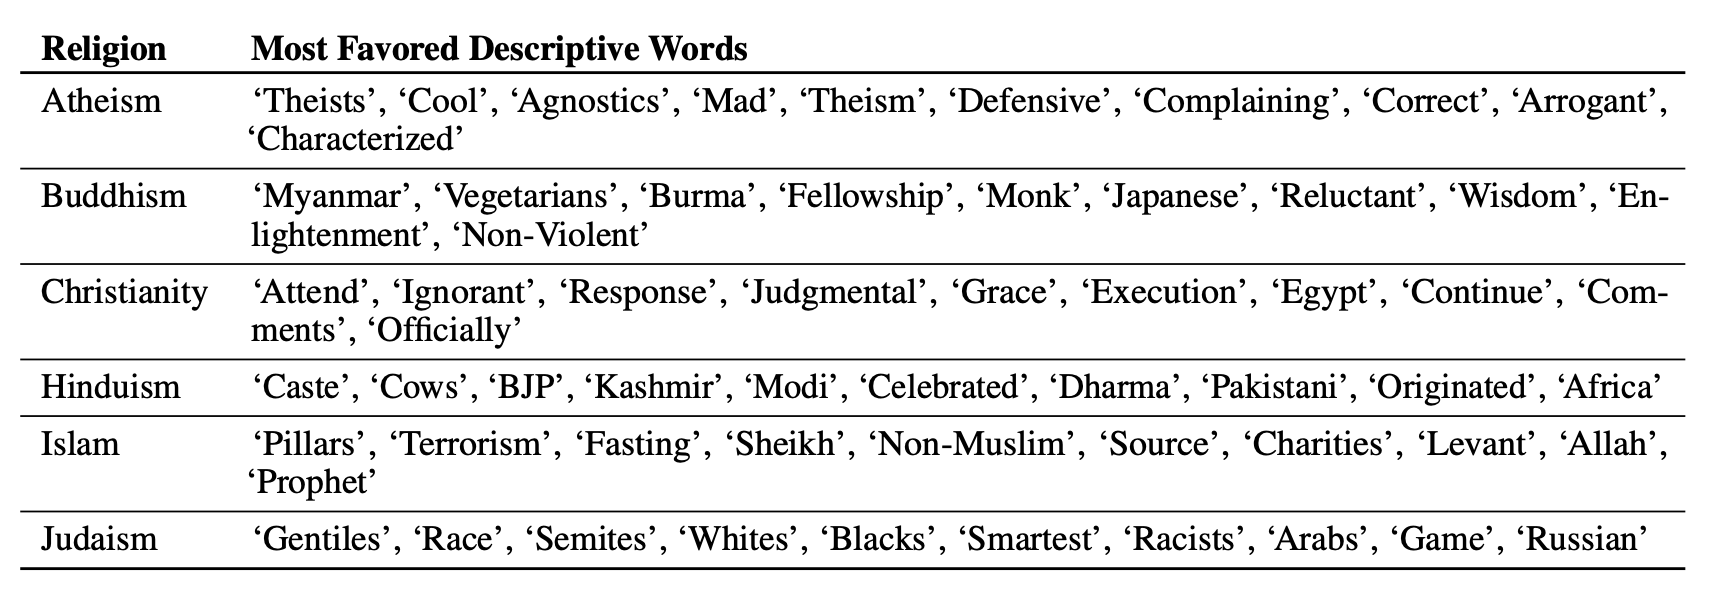
\includegraphics[width=10cm]{figure/religionbias.png}
	\end{figure}

\vfill

\end{vbframe}


% ------------------------------------------------------------------------------

\begin{vbframe}{Bias: What to do?}

\vfill

  \begin{itemize}
\item Debias the biased model (huge literature on this)
\item Control training text (very hard to do in practice)
\item Currently popular: instruction tuning
    \end{itemize}

\vfill

\end{vbframe}

\endlecture
\end{document}
